\documentclass[../main.tex]{subfiles}

\begin{document}
We will begin this section by defining two classes of functions;
the \textit{Partial Recursive Functions} and  the \textit{Turing Computable
Functions}. These two classes of functions give rise to the same class of
functions. The idea behind these two classes of functions is to define what
we intuitively mean with a computable function. The proofs in this section will
be rather informal. The goal of this section will be to state and prove
Kleene's recursion theorem, which will play a crucial role in our proof of 
Solovay's two  completeness theorems.

The topic I have chosen to call \textit{recursion theory} is today often known as
\textit{computability theory}. In his
book \parencite{Soare2016}, Robert Soares has put forth, some arguments for why
this named is better suited for the discipline than recursion theory.

This chapter will follow \citet{Soare1987}, unless stated otherwise. 

\section{Partial Recursive Functions and Recursive Functions}
The class of partial recursive functions is an enlargement of the primitive recursive
functions. The class of primitive recursive functions captures a lot of the
functions we intuitively see as computable. It does not contain any functions that
we would say was incomputable.

But the primitive recursive functions do not include all intuitively computable
functions. For example the following function, called the Ackermann function,
which is clearly computable, is not
in the class of primitive recursive functions:
\begin{align*}
	Ack(0,n)&=n+1\\
	Ack(m+1,0)&=A(m,1)\\
	Ack(m+1,n+1)&=A(m,A(m+1,n))
\end{align*}

This function grows too fast to be a primitive recursive function, i.e
we have for all primitive recursive functions $f(x)$ that for some $y$ that
$Ack(x,y)>f(x)$ for all $x\in \omega$. 
proof of this fact can be found in \citet{Kleene1952}

For the definition of the partial recursive functions we will need the
following operator:
\begin{defi}
	For an expression $P$ we will define $\mu x [P(x)]$ as "the least $x$
	such that $P(x)$".
\end{defi}
So we will need to expand our class of functions, if we want to
\textit{capture} all intuitively computable functions. 
We will expand them in the following way:
\begin{defi}
		The class of \textit{partial recursive} (from now on some times
		called (p.r) functions is the least class closed under schemata
		I through V from the definition of primitive recursive
		(definition \ref{def:Recur})
		functions and the following VI schema. 
		\begin{enumerate}[label=\Roman*., start=6]
			\item If $\theta(\x,y)$ is a partial recursive function
				of $n+1$ variables and 
				\begin{align*}
					\psi(\x)=\mu
					y&[\theta(\x,y)\downarrow=0\\
						&\wedge \forall z\leq y
					[\theta(\x,z)\downarrow]
				\end{align*}
				Then $\psi$ is a partial recursive function of
				$n$ variables.
		\end{enumerate}
		A partial recursive function that is total (define on all of
		$\omega$) is called a total
		recursive function; abbreviated to recursive function.
\end{defi}

This is one way in which one can define what the computable functions are. In
the next section we will present another definition of a type of functions,
and it will be shown that these lead to the same class of functions.

We will end this section with the following definition:
\begin{defi}
	A relation $R\subset\omega^n$ where $n\geq 1$ is \textit{recursive} (primitive
	recursive) if its characteristic function $\chi_R$ is recursive
	(primitive recursive). The case where $n=1$ is the case where $R$ is a
	set $A\subset\omega$, so we also have the definition of a set being
	recursive.
\end{defi}

\section{Turing Computable Functions}

Another way to describe the intuitively computable functions is via a Turing
machine. 
\begin{defi}
	A \textit{Turing machine} $M$ consists of a two-way infinite tape that
	is divided into different cells and a finite set of internal states $Q=\{
	q_0,\ldots, g_n\}$, $n\geq 1$. Each cell  is either blank: B or has
	value 1.
	The following three things can happen simultaneously in a single
	step:
	\begin{enumerate}
		\item Change from one state to another.
		\item Change the scanned symbol $s$ to another symbol
			$s'\in S=\{1,B\}$
		\item Move the reading head one cell to the right (R) or the left
			(L).
	\end{enumerate}
	The operation of $M$ is controlled by a partial map:
	$$\delta:Q\times S\rightarrow Q\times S\times\{R,L\}$$
	Which may not be defined for all arguments.
\end{defi}
The situation can be seen in the following figure:
\begin{center}
	\begin{figure}[h]
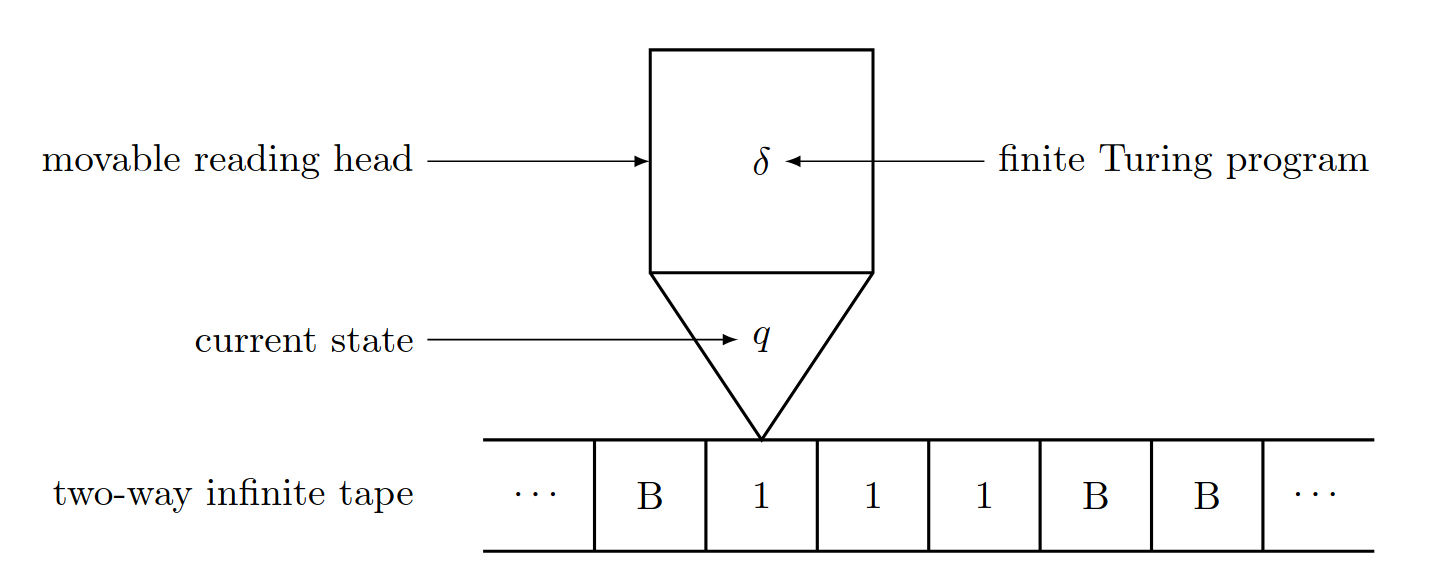
\includegraphics[width=\textwidth]{Turnig.png}
\caption[asd]{A Turing Machine\footnotemark}
\end{figure}
\end{center}
\footnotetext{This picture is taken from \citet{Soare1987}}
The way to understand this definition is the following: if
$(q,s,q',s',X)\in\delta$, it means that the machine $M$ is in stage $q$ where it
scans symbol $s$ then changes to state $q'$ and replaces $s$ by $s'$. Lastly it
moves to the right if $X=R$ and the left if $X=L$. The map $\delta$ is called a
Turing program (denoted by $P$) if it can be viewed as a finite set of quintuples. If the input
integer is $x$ then it will be represented by a string of $x+1$ consecutive
$1's$, where all other cells are blank.

Further the machine $M$ starts in the state $q_1$ by scanning the leftmost cell
that contains a $1$. The machine stops if it reaches the halting state $q_0$,
and it will then output the number $y$, which is the total number of $1$'s on
the tape in this state. If $M$ with input $x$ halts and outputs $y$ we,
say that $M$ computes the partial function $\psi(x)=y$.

The conditions at $M$ for each step of a Turing calculation is determined by
the following:

\begin{enumerate}
	\item The current state $q_i$.
	\item The symbol $s_0$ that is being scanned.
	\item The symbols on the tape to the right of $s_0$ up to the last $1$.
		Denote this sequence by $s_1,s_2,\ldots s_n$
	\item The symbols on the tape to the left of $s_0$ op to the first $1$.
		Denote this sequence by $s_{-1},s_{-2},\ldots s_{-m}$.
\end{enumerate}
This is called the configuration of the machine and we can write it as follows:
$$s_{-m}\cdots s_{-1}q_0s_0s_1\cdots c_n$$

\begin{defi}
	A \textit{Turing computation} according to the Turing program $P$ with input
	$x$ is a sequence of configurations $c_0,c_1,\ldots, c_n$ such that
	$c_0$ represents the machine in the halting state $q_0$, and the
	transition $c_i\rightarrow c_{i+1}$ for all $i<n$ is given by the
	Turing program $P$.
\end{defi}

These definitions makes it possible to list all the Turing programs, by giving
them a Gödel number. This is because each Turing program is a finite set of
quintuples, and thus we can effectively find its Gödel number on a list. We
will now show how to give each Turing program a Gödel number:

\begin{prop}
	Each Turing program $P_e$ can be assigned a Gödel number $e$.
\end{prop}
\begin{proof}
	We will use the fact that each $x\in\omega$ has a unique
	prime decomposition:
	$$x=p_0^{x_0}\cdots p_n^{x_n}\cdots$$
	We can assign a number to each quintuple $(q_i,_j,q_k,s_l,r_m)$ in a
	Turing program $P$ in the following way:
	$$p_0^{1+i}p_1^{1+j}p_2^{1+k}p_3^{1+l}p_4^{1+m}$$
	Where we have that $r_0=R$ and $r_1=L$. 

	Since the prime decomposition
	is unique, each different state of the program has a unique code. Each Turing
	is a sequence of different states and we can thus for an arbitrary
	Turing program $P_e$ let $e_0,\ldots e_n$ denote the Gödel number of
	each different state and set:
	$$e=p_0^{e_0}\cdots p_n^{e_n}$$
	Thus each Turing program $P_e$ has a unique Gödel number $e$.
\end{proof}
Since each Turing program has a unique code we can list them and be able to
find any program $P_e$ by its code $e$. This gives the following definition:
\begin{defi}
	Let $P_e$ be the Turing program with Gödel number $e$ in the list and
	let $\varphi_e^{(n)}$ be the function of $n$ variables computed by $P_e$.
	Further let $\varphi_e$ abbreviate $\varphi_e^{(1)}$.
\end{defi}
\section{The \textit{s-m-n}-Theorem}

It can be proven that the two classes of functions; partial recursive and Turing
computable functions give rise to the same class of partial functions. This
can be seen as evidence for \textit{Church's Thesis}, which states that this
class of functions coincides with the function that we see as intuitively
computable. In the rest of this project we will assume that Church's Thesis
is true. There are some other definitions of computable functions that gives
rise to exactly the same class of functions; a list of these can be found in
\citet{Cutland1980}. This can be seen as further evidence of the correctness of
Church's Thesis; but the thesis cannot be proven, since it is not possible to
rigorously define the notion of an intuitively computable function.

We will begin by proving the padding lemma, which states that each partial
function $\varphi_x$ has an infinite amount of indices.
\begin{lem}[The Padding Lemma]
	Each partial recursive function $\varphi_x$ has $\aleph_0$ indicies,
	and for each $x$ we can \textit{effectively} find an infinite set $A_x$
	of indices for the same partial function.
\end{lem}
\begin{proof}
	For any program $P_x$ that has internal states: $\{q_0,\ldots, q_n\}$
	we can add extra instructions $q_{n+1}B\ R ,q_{n+2}B\ R,\ldots$ such
	that we get a new program for the same computation.
\end{proof}

The following theorem will show that each Turing computable function is in fact
partial recursive. The converse also holds, and the proof of this fact can be
found in \citet{Kleene1952}. The proof of that fact is left out since it is
very tedious.

\begin{thm}[The Normal Form Theorem]
	\label{thm:Normalform}
	There exists a predicate $T(e,x,y)$ and a function $U(y)$ that are
	primitive recursive such that:
	\[\varphi_e(x)=U(\mu yT(e,x,y))\]
\end{thm}
The proof will not be fully rigorous.
\begin{proof}[Proof sketch]
	It can be  shown that the predicate $T(e,x,y)$ exists and is primitive
	recursive, we will only do a bit of this work. This predicate informally
	states that $y$ is the code of Turing program $P_e$ with input $x$. For
	each possible configuration $c$, we can assign a code:
	\[\Godelnum{c}=2^{1+i}\cdot 3^{1+\Godelnum{s_0}}\cdot 5^r\cdot7^l\]
	Where $\Godelnum{s}=0$ if $s=B$ and is equal to $1$ otherwise, $r=\prod_{j\geq
	1}p_j^{\Godelnum{s_j}}$ and $l=\prod_{j\leq -1}p_j^{\Godelnum{s_j}}$.


	 We can now define the code of a Turing computation
	$c_0,c_1,\ldots c_n$ according to $P_e$ to be:
	\[y=2^e\prod_{i\leq n}p_{i+1}^{\Godelnum{s_i}}\]
	From this it follows that $T(e,x,y)$ is computable in the intuitive
	sense.

	Having defined the predicate $T$ we can check if it holds. By
	proposition 2.1 we can "recover" the program $P_e$ from $e$. Then we
	can recover the computation $c_0,c_1,\ldots c_n$ from $y$, if $y$ codes
	such a thing. We can now check if $c_0,c_1,\ldots,c_n$ is a computation
	according to $P_e$ with $x$ as the input in the first configuration
	$c_0$. If this is true, then $U(y)$ just outputs the number of $1$'s in
	the final configuration $c_n$. 

	Further the encoding we have made makes it so that $T$ and $U$ are
	primitive recursive. This is shown in \citet{Kleene1952} on page 376,
	for a flighty different defined predicate $T$.
\end{proof}
This theorem also gives us that each partial recursive function can be created
by two primitive recursive functions, with a single application of the
$\mu$-operator.

\begin{thm}[Enumeration Theorem]
	\label{thm:Emu}
	There is a partial recursive function of $2$ variables
	$\varphi_z^{(2)}(e,x)$ such that $\varphi_z^{(2)}(e,x)=\varphi_e(x)$.
\end{thm}
\begin{proof}
	By Theorem \ref{thm:Normalform} we will define
	$\varphi_z^{(2)}(e,x)=U(\mu y T(e,x,y))=\varphi_e(x)$
\end{proof}
We will need the following notation in the next proof:
\begin{defi}
	Set $\la x,y\ra$ to be the image of $(x,y)$ under the injective
	recursive  pairing function:
	$$\frac{1}{2}(x^2+2xy+y^2+3x+y)$$
	This function is from $\omega\times\omega$ onto $\omega$.
\end{defi}
We can now state and prove the important $s-m-n$ theorem:
\begin{thm}[$s-m-n$ Theorem]
	For every $m,n\geq 1$ there exists an injective recursive function
	$s_n^m$ of $m+1$ variable such that for all $x,y_1,\ldots,y_m$
	\[\varphi^{(n)}_{s^m_n(x,y_1,\ldots,y_m)}(z_1,\ldots z_n)=
	\varphi^{(m+n)}_x(y_1,\ldots,y_m,z_1,\ldots,z_n)\]
\end{thm}
\begin{proof}[Proof sketch]
	I will follow Soare and only prove the case where $m=n=1$. I.e the case
	where we have to prove:
	\[\varphi_{s^1_1(x,y)}(z)=[\varphi_x^{2}(y,z)]\]
	Let $x$ and $y$ be given. Then $s^1_1(x,y)$ can be described as
	follows:
	\begin{enumerate}
		\item Let $P_x$ be the Turing program with code $x$.
		\item Change $P_x$ into another Turing program $P_{x'}$ such
			that: $P_{x'}$ writes $y+1$ "1" left of the input, such
			that there is a B between these 1 and the other input.
			Further i places the head to the left of the new input
			and proceeds to \textit{run} $P_x$.
		\item outputs $x'$
	\end{enumerate}
	it is clear that $P_{x'}$ on input $z$ compute the same as $p_e$ would
	on input $(x,y)$; i.e $\varphi_{x'}=\varphi_x^{(2)}(y,z)$. Further we
	have that $x'=s^1_s(x,y)$.
	By Church's Thesis the function $s=s^1_1$ is recursive, since it can be
	computed effectively. If it is not injective it can be replaced by an
	injective recursive function $s'$ such that
	$\varphi_{s(x,y)}=\varphi_{s'(x,y)}$ by using the padding lemma and by
	defining $s'(x,y)$ in increasing order of $\la x,y\ra$.
\end{proof}

A full proof of this statement can be found in Kleene. The $s-m-n$ theorem
plays a crucial role in both the proof and the use of the recursion theorem.
The theorem is not the most intuitive to use, and takes a bit of work to get
used to. Therefore we will use the $s-m-n$ theorem to
prove the following proposition:
\begin{prop}
	There is a recursive function $g$ of two variables such that for all
	$x,y$:
\[\varphi_{g(x,y)}=\varphi_x\varphi_y\]
\end{prop}
\begin{proof}
	By Church's Thesis it is clear that $\eta=\varphi_x\varphi_y$ is a
	partial recursive function since it is the product of two partial
	recursive functions.

	To end the proof we must show that we can the find Gödel number for $\eta$
	in an uniform effective way from $x$ and $y$ as $x$ and $y$ vary. We
	will begin by defining:
	\[\theta(x,y,z)=\varphi_x(\varphi_y(z))=\varphi_{x_1}(x,\varphi_{x_1}(y,z))\]
	Where $\varphi_{x_1}$ is the function $\varphi_z^{(2)}$ from Theorem
	\ref{thm:Emu}.

	By the Church thesis this function is partial recursive
	and has an index $e$. So by applying the $s-m-n$ Theorem we get:
	\[\varphi_x\varphi_y(z)=
	\varphi_e(x,y,z)=\varphi_{s_1^2(e,x,y)}\]
	And thus $s_1^2(e,x,y)$ is our $g$.
\end{proof}

\section{Recursively Enumerable Sets and the Graph of a Function}
In this section we will introduce the two concepts \textit{recursive
enumerable} sets and the \textit{graph} of a function. We will further show
that there is a connection between these two concepts.

We will first need the following definition before we can define the notion of
recursively enumerable set:

\begin{defi}
	We write $\varphi_{e,s}(x)=y$ if $x,y,e<s$ and $y$ is the output of
	$\varphi_e(x)$ in less than $s$ steps of the Turing program $P_e$.
\end{defi}

The idea behind a recursively enumerable set is that we can have an algorithm
that can enumerate the members of the set.

\begin{defi}
	A set $A$ is \textit{recursively enumerable} (r.e.) if $A$ is the domain of some
	partial recursive function. Further we define the following two sets:
	\begin{enumerate}
		\item We let the $e$th r.e set be denoted by:
			\[E_e=\text{dom}\ (\varphi_e)= \{x:\varphi_e(x)\downarrow\}=\{x:\exists
			y T(e,x,y)\}\]
		\item \[E_{e,s}=\text{dom} (\varphi_{e,s})\]
	\end{enumerate}
\end{defi}
A set can be recursively enumerable without being recursive, which the
following two propositions shows:
\begin{prop}
	Let $K=\{x:\varphi_x(x)\ \text{converges}\}=\{x:x\in E_x\}$, then $K$
	is r.e.
\end{prop}
\begin{proof}
	We have that $K$ is the domain of the following partial recursive
	function:
	\[\psi(x)=\begin{cases}
		x &\text{if}\ \varphi_x(x)\ \text{converges}\\
		\text{undefined} &\text{otherwise.}
	\end{cases}\]
	This function is partial recursive by Church's Thesis, since $\psi(x)$
	can be computed by program $P_x$ on input $x$, which outputs $x$ only
	if $\varphi_x(x)$ converges.
\end{proof}
\begin{prop}
	$K$ is not recursive.
\end{prop}
\begin{proof}
	If $K$ was recursive we would have that it had a recursive characteristic
	function $\chi_K$, and thus the following would be recursive:
	\[f(x)=\begin{cases}
		\varphi_x(x)+1 & \text{if } x\in K\\
		0 & \text{if } x\not \in K
	\end{cases}\]
	But this $f$ can not be recursive, since for all $x$ we have $f\not
	=\varphi_x$.
\end{proof}

So even though we have a algorithm that can enumerate all the members of the
set $K$, we can not for a given $x$ decide whether $x\in K$, so we can not
solve for a given $x$ that $\varphi_x(x)$ converges or not.

The next goal is to show that the definition of a r.e sets is equivalent to the
definition that there is an algorithm that enumerates the members of it. We
will further also show that the definition of a r.e set is equivalent to the
set being $\Sigma_1$, which is a concepts that will play a bigger role later on
in this project.
\begin{defi}
	A set $A$ is the \textit{projection} of some relation $R\subseteq
	\omega\times\omega$ if $A=\{x:\exists y: R(x,y)\}$. We further say that
	a set $A$ is in $\Sigma_1$ form, if $A$ is the projection of some
	recursive relation $R\subseteq\omega\times\omega$.
\end{defi}
We can now show the following theorem:
\begin{thm}[Normal Form Theorem for r.e sets]
	A set $A$ is r.e iff $A$ is $\Sigma_1$.
\end{thm}
\begin{proof}
	($\Rightarrow$) Since $A$ is r.e we have that $A=W_e=\text{dom} \varphi_e$
	for some $e$. This means that:
	$$x\in E_e\Leftrightarrow\exists s(x\in E_{e,s})\Leftrightarrow \exists
	s(T(e,x,s))$$
	Since the relation $T$ is primitive recursive and we have that the set $A$
	is the projection a recursive relation.

	($\Leftarrow$) Let $A=\{x:\exists y(Rx,y)\}$ where $R$ is recursive. We
	then have that $A=\text{dom} (\psi)$ where $\psi(x)=\mu y(R(x,y))$ and thus $A$
	is r.e
\end{proof}
This theorem is equivalent to the normal form theorem for partial recursive
functions. The next theorem shows a way to determine whether a given set is
$\Sigma_1$.
\begin{thm}[Qunatifier Contraction Theorem]
	\label{thm:RecSigma}
	If there is a recursive relation $R\subseteq\omega^{n+1}$ and if we
	have the following set:
	$$A=\{x:\exists y_1\ldots\exists  y_n R(x,\y)\}$$
	Then the set $A$ is $\Sigma_1$.
\end{thm}
\begin{proof}
	We will start of by defining the relation $S\subseteq\omega^2$ as
	follows:
	$$S(x,z)\Leftrightarrow R(x,(z)_1,\ldots,(z)_n)$$
	Where we have the following prime decomposition of $z$:
	$$z=p_1^{(z)_1}\cdots p_k^{(z)_k}$$
	Then the following equivalences hold:
	\begin{align*}
		\exists zS(x,z)&\Leftrightarrow \exists z R(x,(z)_1,\ldots
		(z)_n)\\
			       &\Leftrightarrow \exists y_1\cdots \exists y_n
			       R(x,\y)
	\end{align*}
	And thus the set $A$ is clearly $\Sigma_1$.
\end{proof}
From this theorem, we can easily get the following corollary:
\begin{cor}
	The projection of an r.e relation is r.e.
\end{cor}

The next definition will also play a role in our proof of Solovay's
completeness theorems.

\begin{defi}
	The graph of a (partial) function $\varphi$ is the relation:
	\[(x,y)\in\ \text{graph} (\varphi)\Leftrightarrow f(x)=y\]
\end{defi}
The relation of a graph can also be seen as a function in the language of
$\PRA$; so we will often denote the graph of a function $\varphi(x)=y$ with the
following notation: $\tau xy$, and say that $(x,y)\in\ \text{graph}(\varphi)$ if and
only if $\tau xy$ is true. We will use this notation in chapter 6, since Smorinsky
uses this notation, and we will follow his book \citet{Smor1985} in that
chapter.

\begin{thm}[Uniformaization Theorem]
	If $R\subseteq\omega^2$ is an r.e relation, then there is a p.r
	function $\psi=\text{sel}$ called the selector function for $R$ such that:
	$$\text{sel}(x)\ \text{is defined}\ \Leftrightarrow\ \exists y(R(x,y))$$
	and if this is the case we have that $(x,f(x))\in R$
\end{thm}
\begin{proof}
	Since $R$ is r.e it is $\Sigma_1$. This means that there is a recursive
	relation $S$ such that $R(x,y)$ holds iff $\exists z (S(x,y,z))$. Thus
	we can define the following p.r function:
	$$\theta(x)=\mu u(S(x,(u)_1,(u)_2))$$
	And now we put $\text{sel}(x)=(g(x))_1$
\end{proof}
It will be the following theorem we will use in our proof later on.
\begin{thm}[Graph Theorem]
	A partial function $\varphi$ is partial recursive iff its graph is recursive
	enumerable.
\end{thm}
\begin{proof}
	($\Rightarrow$) The graph of $\varphi_e$ is r.e by theorem \ref{thm:RecSigma} and the
	definition of a graph.

	($\Leftarrow$) Since the graph of $\varphi$ is assumed to be r.e we can
	conclude that $\varphi$ is its own primitive recursive selector function. This
	is that $R=\text{graph} (\varphi)$ can only have $\varphi$ as its selector function.
\end{proof}

We will end this section with the next theorem. It justifies the notion of a
r.e set $A$ as one where we can effectively enumerate its members;
$A=\{a_0,a_1,a_2,\ldots\}$

\begin{thm}[Listning Theorem]
	A set $A$ is r.e if and only if $A=\emptyset$ or $A$ is in the range of
	a total recursive function $f$. 
\end{thm}
\begin{proof}
	($\Leftarrow$) If $A=\emptyset$ then $A$ is clearly r.e. Now
	assume that $A=\text{im}(f)$, where $f$ is a total recursive function. Then
	$A$ is r.e by corollary 2.1

	($\Rightarrow$)
	Let $A=E_e=\emptyset$. We will find the least integer $\la a,t\ra$ such
	that $a\in E_{e,t}$. We will now define the following recursive
	function $f$ as:
	\[f(\la s,x\ra)=\begin{cases}
		x &\ \text{if}\ x\in E_{e,s-1}\setminus E_{e,s}\\
		a &\ \text{otherwise}
	\end{cases}\]
	We have that $A= \text{im} (f)$, since if $x\in E_e$, we can choose the least
	$s$ such that $x\in E_{e,s+1}$, and thus $f(\la s,x\ra)=x$ and hence
	$x\in im(f)$
\end{proof}

\section{The Recursion Theorem}
In this section we will state and prove the recursion theorem. It will be
crucial in chapter 6, since we will need it to define a function, which will be
used to embed a Kripke model into \PRA.
\begin{thm}[The Recursion Theorem]
	For every recursive function $f$ there exists a fixed point $n$ such
	that $\varphi_n=\varphi_{f(x)}$
\end{thm}
\begin{proof}
	We will start of be defining the following \textit{diagonal} function
	$d(u)$ as:
	\begin{align}
		\label{eq:du}
		\varphi_{d(u)}(z)=\begin{cases}
		\varphi_{\varphi_u(u)}(z)& \text{if}\ \varphi_u(u)\
		\text{converges}\\
		\text{undefined} & \text{else}
	\end{cases}
	\end{align}
	By the $s-m-n$ theorem we have that the function $d$ is injective and
	total. Further it is clearly seen that $d$ is independent of $f$.

	Given an arbitrary $f$ we will choose an index $v$ such that:
	\begin{align}
		\label{eq:fd}
		\varphi_v=f\circ d
	\end{align}
	Now set $n=d(v)$. We will show that this is a fixed point for the
	function $f$. Since $f$ is total we also have that $f\circ d$ is total.
	This means that $\varphi_v(v)$ converges and that
	$\varphi_{d(v)}=\varphi_{\varphi_v(v)}$. Thus we have:
	\[\varphi_n=\varphi_{d(v)}=\varphi_{\varphi_v(v)}=\varphi_{f\circ
	d(v)}=\varphi_{f(n)}\]
	The second equality sign follows from \ref{eq:du} and the third follows
	from \ref{eq:fd}.
\end{proof}
Following \citet{Owen1973}, the argument in the proof can be seen as a
digitalization argument that fails. Commonly when we apply a digitalization
argument, we have a class of sequences, with terms from a set $A$, that we arrange as the rows in a square
matrix. We then have a map $h:A\rightarrow A$ that induces an operation $h^*$ on
the set of sequences such that if $\la s(i),i\in I\ra$ is a sequence in our
matrix then 
\[h^*(\la s(i),i\in I\ra)=\la h(s(i)),i\in I\ra\]
After having defined this map we will use it on the sequences that consist of
the elements of the  diagonal of the matrix and
show that the resulting sequence is not one of the original sequences. 

The digitalization argument "fails" in our case, since the sequences of the
diagonal is already one of the rows and thus the image $h^*$ of this
sequences will also be one of the rows; i.e the $h$ has a fixed point.

The start of the proof can be seen as the following lemma:
\begin{lem}
	There is a diaognal function $d(u)$ such that:
	\begin{align}\varphi_{d(u)}(z)=\begin{cases}
		\varphi_{\varphi_u(u)}(z)& \text{if}\ \varphi_u(u)\
		\text{converges}\\
		\text{undefined} & \text{else}
	\end{cases}
	\end{align}
\end{lem}

Most of the time where one uses the Recursion Theorem, one actually uses this
lemma to construct the given function.

\subsection{Application of the Recursion Theorem}
The recursion theorem is a "powerful" tool. It enables us to define a partial
recursive function, which uses its own index as part of its definition. 
The recursion theorem overrides this "self-reference", because we are using the
$s-m-n$ theorem to define a function $f(x)$ and
$\varphi_{f(x)}(z)=(\ldots,x\ldots)$ and then taking a fixed point:
$\varphi_n=\varphi_{f(n)}$.  When we are making constructions like this, the
only thing we cannot do is use specific properties of the function $\varphi_n$.
We will use the theorem in this way in our proof of Solovay's completeness
theorems to define a function with the help of the function own Gödel number; and
the recursion theorem makes this a viable tactic.

The
following examples will show a few uses of this theorem.
\begin{exmp}
	We will show that there is an $n$ such that:
	$$W_n=\{n\}$$
	We start of by using the $s-m-n$ theorem to define $W_{f(x)}=\{x\}$,
	then by the recursion theorem we can choose $n$ such that we have:
	$$W_n=W_{f(n)}=\{n\}$$
\end{exmp}

The next example will be an application of the Recursion Theorem that is in the
same vein as the one we will use for proving Solovay's completeness
theorems.
\begin{exmp}
	Let $\psi:\omega^2\rightarrow\omega$ and
	$\theta:\omega^3\rightarrow\omega$ be recursive functions and define
	the function $\varphi:\omega^2\rightarrow\omega$ by:
	\begin{align*}
		\varphi(0,y)&=\psi(y)\\
		\varphi(x+1,y)&=\theta(\varphi(x,y),x,y)
	\end{align*}
	We will now show that $\varphi$ is recursive by using the recursion
	theorem.

	Let $\tau_0 v_0v_1$ be an arbitrary graph and let $\tau_1v_0v_1$ be the
	graph of $\psi$ and $\zeta v_0v_1v_2$ be the graph of $\theta$. We will
	now look at the following formula:
	\[\Xi(\tau_0):\ (v_0=\0\wedge \tau_1v_0v_1)\vee (v_0>\0\wedge \exists
	v(\tau_0(v_+-1,v)\wedge \zeta vv_0v_1))\]
	We can see $\Godelnum{\Xi(\tau_0)}$ as a primitive recursive function
	representing  $\Godelnum{\tau_0}$. I.e we have:
	\[\Godelnum{\Xi(\tau_0)}=\eta(\Godelnum{\tau_0})\]
	We can now use the Recursion Theorem to chose an $n$ such that we have:
	$\varphi^{(2)}_{\eta(n)}=\varphi^{(2)}_n$ and for
	$\varphi=\varphi^{(2)}_n$ we have:
	\[\varphi(x,y)=z\leftrightarrow(x=0\wedge\psi(y)=z=\vee(x>0\wedge
	\theta(\varphi(x-1,y),x,y)=z)\]
	I.e $\varphi$ does exactly what we want it to do. We just need to
	define $\varphi$ and this can be done by a $\Sigma_1$ induction.
\end{exmp}

This end our discussion about recursion theory. In the next chapter, we will
generalize the notion of $\Sigma_1$ sets and in chapter \ref{chap:Complete} we
will use the recursion theorem to define the  function that we will use to
embed a Kripke model into \PRA.

\end{document}
